\documentclass[twoside]{book}

% Packages required by doxygen
\usepackage{fixltx2e}
\usepackage{calc}
\usepackage{doxygen}
\usepackage[export]{adjustbox} % also loads graphicx
\usepackage{graphicx}
\usepackage[utf8]{inputenc}
\usepackage{makeidx}
\usepackage{multicol}
\usepackage{multirow}
\PassOptionsToPackage{warn}{textcomp}
\usepackage{textcomp}
\usepackage[nointegrals]{wasysym}
\usepackage[table]{xcolor}

% NLS support packages
\usepackage[french]{babel}

% Font selection
\usepackage[T1]{fontenc}
\usepackage[scaled=.90]{helvet}
\usepackage{courier}
\usepackage{amssymb}
\usepackage{sectsty}
\renewcommand{\familydefault}{\sfdefault}
\allsectionsfont{%
  \fontseries{bc}\selectfont%
  \color{darkgray}%
}
\renewcommand{\DoxyLabelFont}{%
  \fontseries{bc}\selectfont%
  \color{darkgray}%
}
\newcommand{\+}{\discretionary{\mbox{\scriptsize$\hookleftarrow$}}{}{}}

% Page & text layout
\usepackage{geometry}
\geometry{%
  a4paper,%
  top=2.5cm,%
  bottom=2.5cm,%
  left=2.5cm,%
  right=2.5cm%
}
\tolerance=750
\hfuzz=15pt
\hbadness=750
\setlength{\emergencystretch}{15pt}
\setlength{\parindent}{0cm}
\setlength{\parskip}{0.2cm}
\makeatletter
\renewcommand{\paragraph}{%
  \@startsection{paragraph}{4}{0ex}{-1.0ex}{1.0ex}{%
    \normalfont\normalsize\bfseries\SS@parafont%
  }%
}
\renewcommand{\subparagraph}{%
  \@startsection{subparagraph}{5}{0ex}{-1.0ex}{1.0ex}{%
    \normalfont\normalsize\bfseries\SS@subparafont%
  }%
}
\makeatother

% Headers & footers
\usepackage{fancyhdr}
\pagestyle{fancyplain}
\fancyhead[LE]{\fancyplain{}{\bfseries\thepage}}
\fancyhead[CE]{\fancyplain{}{}}
\fancyhead[RE]{\fancyplain{}{\bfseries\leftmark}}
\fancyhead[LO]{\fancyplain{}{\bfseries\rightmark}}
\fancyhead[CO]{\fancyplain{}{}}
\fancyhead[RO]{\fancyplain{}{\bfseries\thepage}}
\fancyfoot[LE]{\fancyplain{}{}}
\fancyfoot[CE]{\fancyplain{}{}}
\fancyfoot[RE]{\fancyplain{}{\bfseries\scriptsize Généré le Mardi 29 Décembre 2015 21\+:00\+:35 pour Color\+Flood par Doxygen }}
\fancyfoot[LO]{\fancyplain{}{\bfseries\scriptsize Généré le Mardi 29 Décembre 2015 21\+:00\+:35 pour Color\+Flood par Doxygen }}
\fancyfoot[CO]{\fancyplain{}{}}
\fancyfoot[RO]{\fancyplain{}{}}
\renewcommand{\footrulewidth}{0.4pt}
\renewcommand{\chaptermark}[1]{%
  \markboth{#1}{}%
}
\renewcommand{\sectionmark}[1]{%
  \markright{\thesection\ #1}%
}

% Indices & bibliography
\usepackage{natbib}
\usepackage[titles]{tocloft}
\setcounter{tocdepth}{3}
\setcounter{secnumdepth}{5}
\makeindex

% Hyperlinks (required, but should be loaded last)
\usepackage{ifpdf}
\ifpdf
  \usepackage[pdftex,pagebackref=true]{hyperref}
\else
  \usepackage[ps2pdf,pagebackref=true]{hyperref}
\fi
\hypersetup{%
  colorlinks=true,%
  linkcolor=blue,%
  citecolor=blue,%
  unicode%
}

% Custom commands
\newcommand{\clearemptydoublepage}{%
  \newpage{\pagestyle{empty}\cleardoublepage}%
}


%===== C O N T E N T S =====

\begin{document}

% Titlepage & ToC
\hypersetup{pageanchor=false,
             bookmarks=true,
             bookmarksnumbered=true,
             pdfencoding=unicode
            }
\pagenumbering{roman}
\begin{titlepage}
\vspace*{7cm}
\begin{center}%
{\Large Color\+Flood }\\
\vspace*{1cm}
{\large Généré par Doxygen 1.8.10}\\
\vspace*{0.5cm}
{\small Mardi 29 Décembre 2015 21:00:35}\\
\end{center}
\end{titlepage}
\clearemptydoublepage
\tableofcontents
\clearemptydoublepage
\pagenumbering{arabic}
\hypersetup{pageanchor=true}

%--- Begin generated contents ---
\chapter{Index hiérarchique}
\section{Hiérarchie des classes}
Cette liste d\textquotesingle{}héritage est classée approximativement par ordre alphabétique \+:\begin{DoxyCompactList}
\item Callback\begin{DoxyCompactList}
\item \contentsline{section}{p8.\+demo.\+p8sokoban.\+Sokoban\+View}{\pageref{classp8_1_1demo_1_1p8sokoban_1_1_sokoban_view}}{}
\end{DoxyCompactList}
\item Runnable\begin{DoxyCompactList}
\item \contentsline{section}{p8.\+demo.\+p8sokoban.\+Sokoban\+View}{\pageref{classp8_1_1demo_1_1p8sokoban_1_1_sokoban_view}}{}
\end{DoxyCompactList}
\item Activity\begin{DoxyCompactList}
\item \contentsline{section}{p8.\+demo.\+p8sokoban.\+p8\+\_\+\+Sokoban}{\pageref{classp8_1_1demo_1_1p8sokoban_1_1p8___sokoban}}{}
\end{DoxyCompactList}
\item Surface\+View\begin{DoxyCompactList}
\item \contentsline{section}{p8.\+demo.\+p8sokoban.\+Sokoban\+View}{\pageref{classp8_1_1demo_1_1p8sokoban_1_1_sokoban_view}}{}
\end{DoxyCompactList}
\end{DoxyCompactList}

\chapter{Index des classes}
\section{Liste des classes}
Liste des classes, structures, unions et interfaces avec une brève description \+:\begin{DoxyCompactList}
\item\contentsline{section}{\hyperlink{classp8_1_1demo_1_1p8sokoban_1_1p8___sokoban}{p8.\+demo.\+p8sokoban.\+p8\+\_\+\+Sokoban} }{\pageref{classp8_1_1demo_1_1p8sokoban_1_1p8___sokoban}}{}
\item\contentsline{section}{\hyperlink{classp8_1_1demo_1_1p8sokoban_1_1_sokoban_view}{p8.\+demo.\+p8sokoban.\+Sokoban\+View} }{\pageref{classp8_1_1demo_1_1p8sokoban_1_1_sokoban_view}}{}
\end{DoxyCompactList}

\chapter{Documentation des classes}
\hypertarget{classp8_1_1demo_1_1p8sokoban_1_1p8___sokoban}{}\section{Référence de la classe p8.\+demo.\+p8sokoban.\+p8\+\_\+\+Sokoban}
\label{classp8_1_1demo_1_1p8sokoban_1_1p8___sokoban}\index{p8.\+demo.\+p8sokoban.\+p8\+\_\+\+Sokoban@{p8.\+demo.\+p8sokoban.\+p8\+\_\+\+Sokoban}}


Graphe d\textquotesingle{}héritage de p8.\+demo.\+p8sokoban.\+p8\+\_\+\+Sokoban\+:
\nopagebreak
\begin{figure}[H]
\begin{center}
\leavevmode
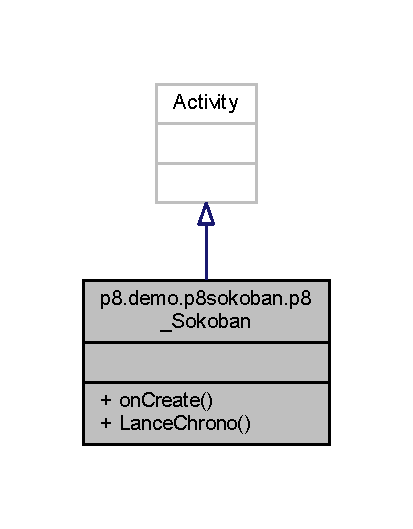
\includegraphics[width=198pt]{classp8_1_1demo_1_1p8sokoban_1_1p8___sokoban__inherit__graph}
\end{center}
\end{figure}


Graphe de collaboration de p8.\+demo.\+p8sokoban.\+p8\+\_\+\+Sokoban\+:
\nopagebreak
\begin{figure}[H]
\begin{center}
\leavevmode
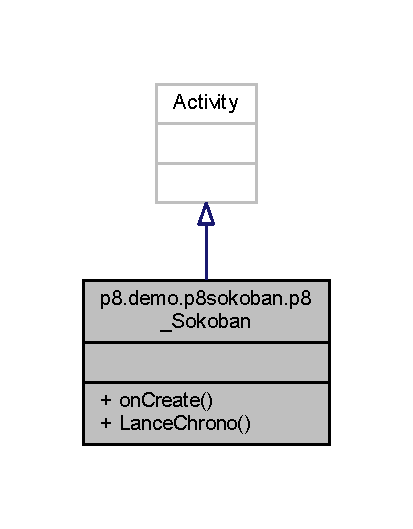
\includegraphics[width=198pt]{classp8_1_1demo_1_1p8sokoban_1_1p8___sokoban__coll__graph}
\end{center}
\end{figure}
\subsection*{Fonctions membres publiques}
\begin{DoxyCompactItemize}
\item 
void \hyperlink{classp8_1_1demo_1_1p8sokoban_1_1p8___sokoban_a4b9ef11394d277a9323ba41d191ebeaf}{on\+Create} (Bundle saved\+Instance\+State)
\end{DoxyCompactItemize}
\subsection*{Fonctions membres publiques statiques}
\begin{DoxyCompactItemize}
\item 
static void \hyperlink{classp8_1_1demo_1_1p8sokoban_1_1p8___sokoban_aba7394226cddb3359f918156472ac556}{Lance\+Chrono} ()
\end{DoxyCompactItemize}


\subsection{Documentation des fonctions membres}
\hypertarget{classp8_1_1demo_1_1p8sokoban_1_1p8___sokoban_aba7394226cddb3359f918156472ac556}{}\index{p8\+::demo\+::p8sokoban\+::p8\+\_\+\+Sokoban@{p8\+::demo\+::p8sokoban\+::p8\+\_\+\+Sokoban}!Lance\+Chrono@{Lance\+Chrono}}
\index{Lance\+Chrono@{Lance\+Chrono}!p8\+::demo\+::p8sokoban\+::p8\+\_\+\+Sokoban@{p8\+::demo\+::p8sokoban\+::p8\+\_\+\+Sokoban}}
\subsubsection[{Lance\+Chrono()}]{\setlength{\rightskip}{0pt plus 5cm}static void p8.\+demo.\+p8sokoban.\+p8\+\_\+\+Sokoban.\+Lance\+Chrono (
\begin{DoxyParamCaption}
{}
\end{DoxyParamCaption}
)\hspace{0.3cm}{\ttfamily [static]}}\label{classp8_1_1demo_1_1p8sokoban_1_1p8___sokoban_aba7394226cddb3359f918156472ac556}
Fonction qui lance le chronometre \hypertarget{classp8_1_1demo_1_1p8sokoban_1_1p8___sokoban_a4b9ef11394d277a9323ba41d191ebeaf}{}\index{p8\+::demo\+::p8sokoban\+::p8\+\_\+\+Sokoban@{p8\+::demo\+::p8sokoban\+::p8\+\_\+\+Sokoban}!on\+Create@{on\+Create}}
\index{on\+Create@{on\+Create}!p8\+::demo\+::p8sokoban\+::p8\+\_\+\+Sokoban@{p8\+::demo\+::p8sokoban\+::p8\+\_\+\+Sokoban}}
\subsubsection[{on\+Create(\+Bundle saved\+Instance\+State)}]{\setlength{\rightskip}{0pt plus 5cm}void p8.\+demo.\+p8sokoban.\+p8\+\_\+\+Sokoban.\+on\+Create (
\begin{DoxyParamCaption}
\item[{Bundle}]{saved\+Instance\+State}
\end{DoxyParamCaption}
)}\label{classp8_1_1demo_1_1p8sokoban_1_1p8___sokoban_a4b9ef11394d277a9323ba41d191ebeaf}
initialise notre activity avec le constructeur parent charge le fichier main.\+xml comme vue de l\textquotesingle{}activite recuperation de la vue une voie cree e partir de son id rend visible la vue


\begin{DoxyParams}{Paramètres}
{\em saved\+Instance\+State} & \\
\hline
\end{DoxyParams}


La documentation de cette classe a été générée à partir du fichier suivant \+:\begin{DoxyCompactItemize}
\item 
app/src/main/java/p8/demo/p8sokoban/p8\+\_\+\+Sokoban.\+java\end{DoxyCompactItemize}

\hypertarget{classp8_1_1demo_1_1p8sokoban_1_1_sokoban_view}{}\section{Référence de la classe p8.\+demo.\+p8sokoban.\+Sokoban\+View}
\label{classp8_1_1demo_1_1p8sokoban_1_1_sokoban_view}\index{p8.\+demo.\+p8sokoban.\+Sokoban\+View@{p8.\+demo.\+p8sokoban.\+Sokoban\+View}}


Graphe d\textquotesingle{}héritage de p8.\+demo.\+p8sokoban.\+Sokoban\+View\+:
\nopagebreak
\begin{figure}[H]
\begin{center}
\leavevmode
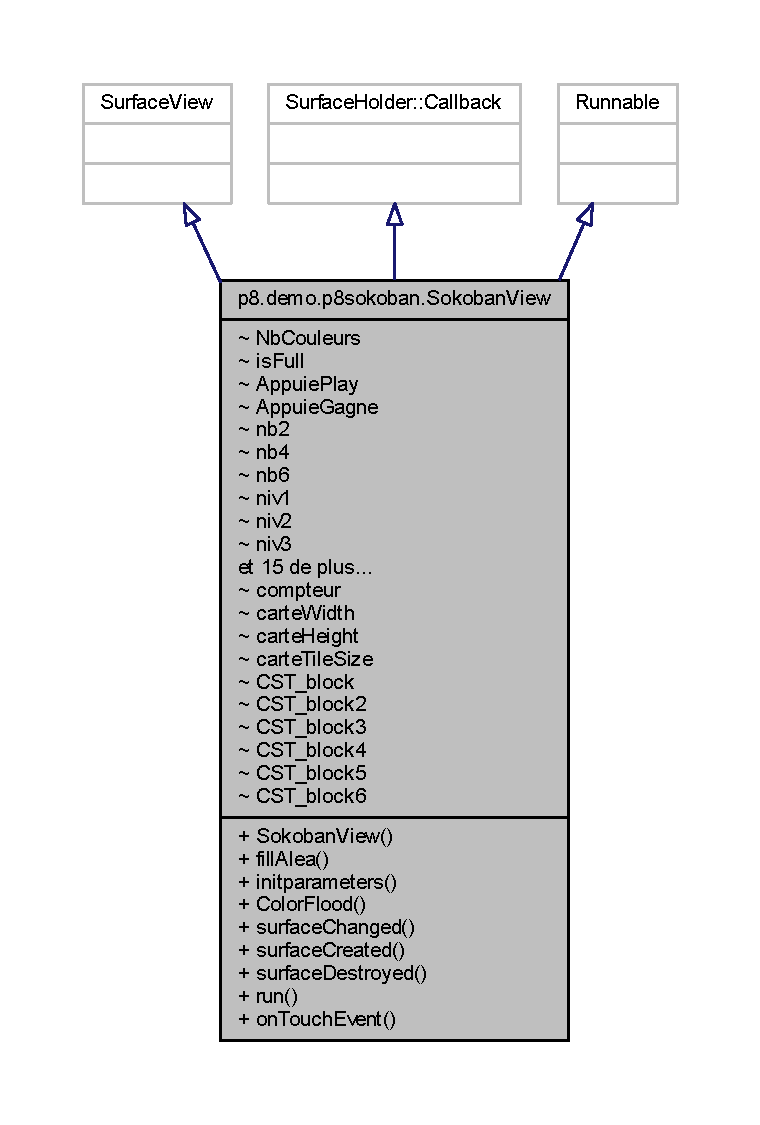
\includegraphics[width=350pt]{classp8_1_1demo_1_1p8sokoban_1_1_sokoban_view__inherit__graph}
\end{center}
\end{figure}


Graphe de collaboration de p8.\+demo.\+p8sokoban.\+Sokoban\+View\+:
\nopagebreak
\begin{figure}[H]
\begin{center}
\leavevmode
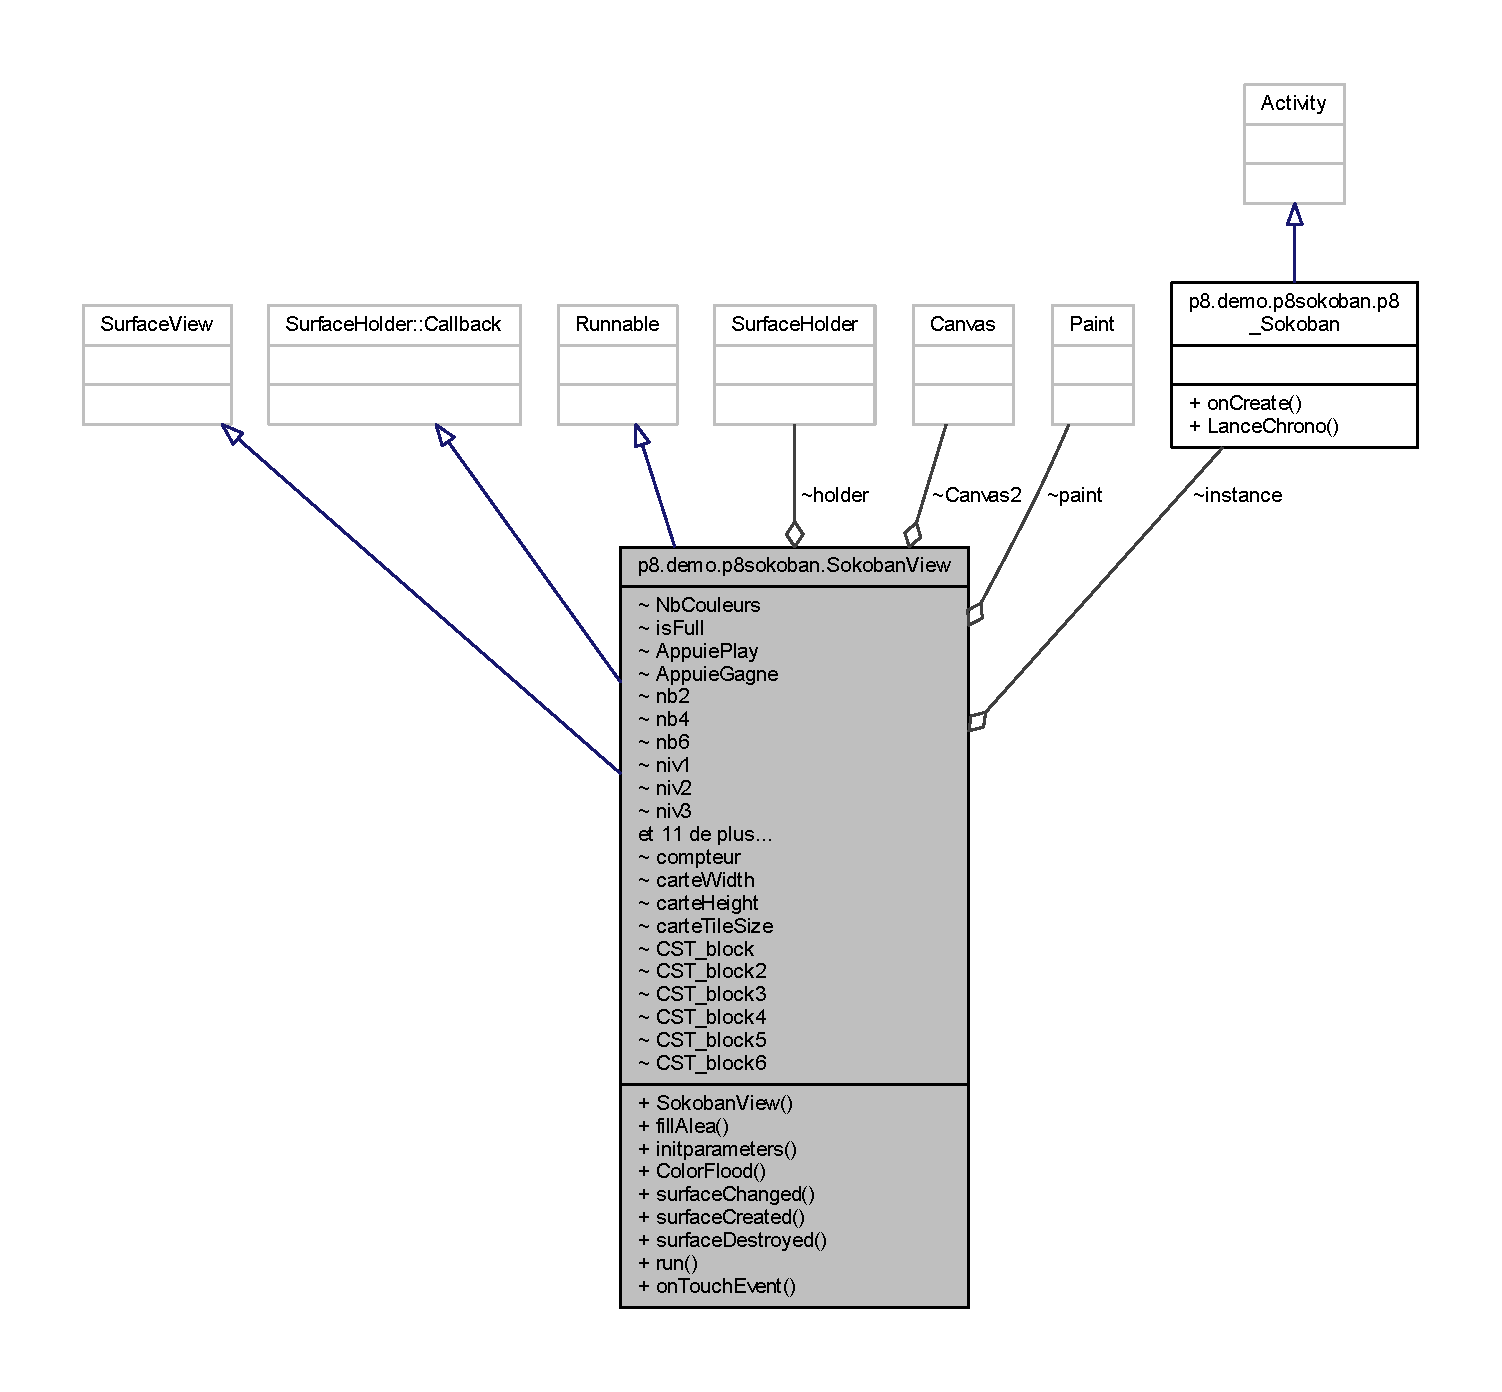
\includegraphics[width=350pt]{classp8_1_1demo_1_1p8sokoban_1_1_sokoban_view__coll__graph}
\end{center}
\end{figure}
\subsection*{Fonctions membres publiques}
\begin{DoxyCompactItemize}
\item 
\hyperlink{classp8_1_1demo_1_1p8sokoban_1_1_sokoban_view_a9b77c402af6779c46c11e0bd6572eeec}{Sokoban\+View} (Context context, Attribute\+Set attrs)
\item 
void \hyperlink{classp8_1_1demo_1_1p8sokoban_1_1_sokoban_view_a69207fcf45a27f3516d24fb087428ae7}{fill\+Alea} (int Nombre\+Couleurs)
\item 
void \hyperlink{classp8_1_1demo_1_1p8sokoban_1_1_sokoban_view_aae2d77f292a6cc7b5e4b68f0c8df0243}{initparameters} ()
\item 
void \hyperlink{classp8_1_1demo_1_1p8sokoban_1_1_sokoban_view_a72d3a3f62698678446745c2ddbddb6aa}{Color\+Flood} (int x, int y, int Old\+Color, int New\+Color)
\item 
void \hyperlink{classp8_1_1demo_1_1p8sokoban_1_1_sokoban_view_a6f555dde84f49e730114c5585e444e2b}{surface\+Changed} (Surface\+Holder holder, int format, int width, int height)
\item 
\hypertarget{classp8_1_1demo_1_1p8sokoban_1_1_sokoban_view_a4b9325992cfbf98b878f11b75909edac}{}void {\bfseries surface\+Created} (Surface\+Holder arg0)\label{classp8_1_1demo_1_1p8sokoban_1_1_sokoban_view_a4b9325992cfbf98b878f11b75909edac}

\item 
\hypertarget{classp8_1_1demo_1_1p8sokoban_1_1_sokoban_view_a0b190fc3dd3e36091c512adb6d827172}{}void {\bfseries surface\+Destroyed} (Surface\+Holder arg0)\label{classp8_1_1demo_1_1p8sokoban_1_1_sokoban_view_a0b190fc3dd3e36091c512adb6d827172}

\item 
void \hyperlink{classp8_1_1demo_1_1p8sokoban_1_1_sokoban_view_a6c6c4a3e01b49c9b46fbf698eda4ad5a}{run} ()
\item 
boolean \hyperlink{classp8_1_1demo_1_1p8sokoban_1_1_sokoban_view_a7447a5c085cc25b6be162b832a358700}{on\+Touch\+Event} (Motion\+Event event)
\end{DoxyCompactItemize}


\subsection{Documentation des constructeurs et destructeur}
\hypertarget{classp8_1_1demo_1_1p8sokoban_1_1_sokoban_view_a9b77c402af6779c46c11e0bd6572eeec}{}\index{p8\+::demo\+::p8sokoban\+::\+Sokoban\+View@{p8\+::demo\+::p8sokoban\+::\+Sokoban\+View}!Sokoban\+View@{Sokoban\+View}}
\index{Sokoban\+View@{Sokoban\+View}!p8\+::demo\+::p8sokoban\+::\+Sokoban\+View@{p8\+::demo\+::p8sokoban\+::\+Sokoban\+View}}
\subsubsection[{Sokoban\+View(\+Context context, Attribute\+Set attrs)}]{\setlength{\rightskip}{0pt plus 5cm}p8.\+demo.\+p8sokoban.\+Sokoban\+View.\+Sokoban\+View (
\begin{DoxyParamCaption}
\item[{Context}]{context, }
\item[{Attribute\+Set}]{attrs}
\end{DoxyParamCaption}
)}\label{classp8_1_1demo_1_1p8sokoban_1_1_sokoban_view_a9b77c402af6779c46c11e0bd6572eeec}
The constructor called from the main Jet\+Boy activity


\begin{DoxyParams}{Paramètres}
{\em context} & \\
\hline
{\em attrs} & \\
\hline
\end{DoxyParams}


\subsection{Documentation des fonctions membres}
\hypertarget{classp8_1_1demo_1_1p8sokoban_1_1_sokoban_view_a72d3a3f62698678446745c2ddbddb6aa}{}\index{p8\+::demo\+::p8sokoban\+::\+Sokoban\+View@{p8\+::demo\+::p8sokoban\+::\+Sokoban\+View}!Color\+Flood@{Color\+Flood}}
\index{Color\+Flood@{Color\+Flood}!p8\+::demo\+::p8sokoban\+::\+Sokoban\+View@{p8\+::demo\+::p8sokoban\+::\+Sokoban\+View}}
\subsubsection[{Color\+Flood(int x, int y, int Old\+Color, int New\+Color)}]{\setlength{\rightskip}{0pt plus 5cm}void p8.\+demo.\+p8sokoban.\+Sokoban\+View.\+Color\+Flood (
\begin{DoxyParamCaption}
\item[{int}]{x, }
\item[{int}]{y, }
\item[{int}]{Old\+Color, }
\item[{int}]{New\+Color}
\end{DoxyParamCaption}
)}\label{classp8_1_1demo_1_1p8sokoban_1_1_sokoban_view_a72d3a3f62698678446745c2ddbddb6aa}
Va changer la couleur de la première case en fonction de la couleur choisi Ensuite on teste si les cases autours d\textquotesingle{}elle sont de la même couleur que l\textquotesingle{}ancienne Si oui on change ses cases à la couleur choisi 
\begin{DoxyParams}{Paramètres}
{\em x} & \\
\hline
{\em y} & \\
\hline
{\em Old\+Color} & \\
\hline
{\em New\+Color} & \\
\hline
\end{DoxyParams}
\hypertarget{classp8_1_1demo_1_1p8sokoban_1_1_sokoban_view_a69207fcf45a27f3516d24fb087428ae7}{}\index{p8\+::demo\+::p8sokoban\+::\+Sokoban\+View@{p8\+::demo\+::p8sokoban\+::\+Sokoban\+View}!fill\+Alea@{fill\+Alea}}
\index{fill\+Alea@{fill\+Alea}!p8\+::demo\+::p8sokoban\+::\+Sokoban\+View@{p8\+::demo\+::p8sokoban\+::\+Sokoban\+View}}
\subsubsection[{fill\+Alea(int Nombre\+Couleurs)}]{\setlength{\rightskip}{0pt plus 5cm}void p8.\+demo.\+p8sokoban.\+Sokoban\+View.\+fill\+Alea (
\begin{DoxyParamCaption}
\item[{int}]{Nombre\+Couleurs}
\end{DoxyParamCaption}
)}\label{classp8_1_1demo_1_1p8sokoban_1_1_sokoban_view_a69207fcf45a27f3516d24fb087428ae7}
Remplir le tableau aleatoirement 
\begin{DoxyParams}{Paramètres}
{\em Nombre\+Couleurs} & \\
\hline
\end{DoxyParams}
\hypertarget{classp8_1_1demo_1_1p8sokoban_1_1_sokoban_view_aae2d77f292a6cc7b5e4b68f0c8df0243}{}\index{p8\+::demo\+::p8sokoban\+::\+Sokoban\+View@{p8\+::demo\+::p8sokoban\+::\+Sokoban\+View}!initparameters@{initparameters}}
\index{initparameters@{initparameters}!p8\+::demo\+::p8sokoban\+::\+Sokoban\+View@{p8\+::demo\+::p8sokoban\+::\+Sokoban\+View}}
\subsubsection[{initparameters()}]{\setlength{\rightskip}{0pt plus 5cm}void p8.\+demo.\+p8sokoban.\+Sokoban\+View.\+initparameters (
\begin{DoxyParamCaption}
{}
\end{DoxyParamCaption}
)}\label{classp8_1_1demo_1_1p8sokoban_1_1_sokoban_view_aae2d77f292a6cc7b5e4b68f0c8df0243}
initialisation du jeu \hypertarget{classp8_1_1demo_1_1p8sokoban_1_1_sokoban_view_a7447a5c085cc25b6be162b832a358700}{}\index{p8\+::demo\+::p8sokoban\+::\+Sokoban\+View@{p8\+::demo\+::p8sokoban\+::\+Sokoban\+View}!on\+Touch\+Event@{on\+Touch\+Event}}
\index{on\+Touch\+Event@{on\+Touch\+Event}!p8\+::demo\+::p8sokoban\+::\+Sokoban\+View@{p8\+::demo\+::p8sokoban\+::\+Sokoban\+View}}
\subsubsection[{on\+Touch\+Event(\+Motion\+Event event)}]{\setlength{\rightskip}{0pt plus 5cm}boolean p8.\+demo.\+p8sokoban.\+Sokoban\+View.\+on\+Touch\+Event (
\begin{DoxyParamCaption}
\item[{Motion\+Event}]{event}
\end{DoxyParamCaption}
)}\label{classp8_1_1demo_1_1p8sokoban_1_1_sokoban_view_a7447a5c085cc25b6be162b832a358700}
fonction permettant de recuperer les evenements tactiles 
\begin{DoxyParams}{Paramètres}
{\em event} & \\
\hline
\end{DoxyParams}
\begin{DoxyReturn}{Renvoie}

\end{DoxyReturn}
\hypertarget{classp8_1_1demo_1_1p8sokoban_1_1_sokoban_view_a6c6c4a3e01b49c9b46fbf698eda4ad5a}{}\index{p8\+::demo\+::p8sokoban\+::\+Sokoban\+View@{p8\+::demo\+::p8sokoban\+::\+Sokoban\+View}!run@{run}}
\index{run@{run}!p8\+::demo\+::p8sokoban\+::\+Sokoban\+View@{p8\+::demo\+::p8sokoban\+::\+Sokoban\+View}}
\subsubsection[{run()}]{\setlength{\rightskip}{0pt plus 5cm}void p8.\+demo.\+p8sokoban.\+Sokoban\+View.\+run (
\begin{DoxyParamCaption}
{}
\end{DoxyParamCaption}
)}\label{classp8_1_1demo_1_1p8sokoban_1_1_sokoban_view_a6c6c4a3e01b49c9b46fbf698eda4ad5a}
run (run du thread cree) on endort le thread, on modifie le compteur d\textquotesingle{}animation, on prend la main pour dessiner et on dessine puis on libere le canvas \hypertarget{classp8_1_1demo_1_1p8sokoban_1_1_sokoban_view_a6f555dde84f49e730114c5585e444e2b}{}\index{p8\+::demo\+::p8sokoban\+::\+Sokoban\+View@{p8\+::demo\+::p8sokoban\+::\+Sokoban\+View}!surface\+Changed@{surface\+Changed}}
\index{surface\+Changed@{surface\+Changed}!p8\+::demo\+::p8sokoban\+::\+Sokoban\+View@{p8\+::demo\+::p8sokoban\+::\+Sokoban\+View}}
\subsubsection[{surface\+Changed(\+Surface\+Holder holder, int format, int width, int height)}]{\setlength{\rightskip}{0pt plus 5cm}void p8.\+demo.\+p8sokoban.\+Sokoban\+View.\+surface\+Changed (
\begin{DoxyParamCaption}
\item[{Surface\+Holder}]{holder, }
\item[{int}]{format, }
\item[{int}]{width, }
\item[{int}]{height}
\end{DoxyParamCaption}
)}\label{classp8_1_1demo_1_1p8sokoban_1_1_sokoban_view_a6f555dde84f49e730114c5585e444e2b}
callback sur le cycle de vie de la surfaceview 
\begin{DoxyParams}{Paramètres}
{\em holder} & \\
\hline
{\em format} & \\
\hline
{\em width} & \\
\hline
{\em height} & \\
\hline
\end{DoxyParams}


La documentation de cette classe a été générée à partir du fichier suivant \+:\begin{DoxyCompactItemize}
\item 
app/src/main/java/p8/demo/p8sokoban/Sokoban\+View.\+java\end{DoxyCompactItemize}

%--- End generated contents ---

% Index
\backmatter
\newpage
\phantomsection
\clearemptydoublepage
\addcontentsline{toc}{chapter}{Index}
\printindex

\end{document}
